\section{Auswertung}
\label{sec:Auswertung}
\subsection{Bestimmung der Fourierkoeffizienten}
\subsubsection{Sägezahnspannung}
Die Funktion der Sägezahnspannung wird folgendermaßen parametrisiert und periodisch fortgesetzt:
\begin{align}
    f(t) = U_0
    \left(1 - \frac{2}{T}\,t\right), \:\:\:\: 0\leq t < T
\end{align}
Da $f(t)$ eine ungerade Funktion ist, folgt sofort $a_n=0$, für alle $n>0$.
Über eine gesamte Periode integriert ist die Funktion 0, woraus folgt, dass $a_0=0$.
Für die $b_n$ folgt nach Gleichung \eqref{eq:sin}:
\begin{equation}
    b_n = \frac{2U_0}{\pi n}
\end{equation}
Es sind die ersten zehn nicht verschwindenden $b_n$ in Tabelle \ref{tab:sägezahnt} angegeben.
\begin{table}
    \centering
    \caption{Fourierkoeffizienten einer Sägezahnspannung.}
    \label{tab:sägezahnt}
    \begin{tabular}{S[table-format=2.0] S[table-format=2.2]}
    \toprule
    {$n$} & {$b_n/\si{\volt}$} \\
    \midrule
    1   & 13.11 \\
    2   & 6.55  \\
    3   & 4.37  \\
    4   & 3.28  \\
    5   & 2.62  \\
    6   & 2.18  \\
    7   & 1.87  \\
    8   & 1.64  \\
    9   & 1.46  \\
    10  & 1.31  \\    
    \bottomrule
    \end{tabular}
\end{table}
\noindent
\subsubsection{Dreieckspannung}
Die Parametrisierung der Dreieckspannung folgt nach:
\begin{equation}
    f(t) = U_0
    \begin{dcases}
        1-\frac{4}{T}\,t,     & 0\leq t < \frac{T}{2} \\
        \frac{4}{T}\,t - 3,   & \frac{T}{2} \leq t < T
    \end{dcases}
\end{equation} 
Die Dreieckspannug ist eine gerade Funktion, weshalb $b_n=0$, für alle $n$.
Auch hier beträgt das Integral über eine ganze Periode 0, woraus folgt $a_0=0$.
Die $a_n$ berechnen sich nach Gleichung \eqref{eq:cos}.
\begin{equation}
    a_n = \frac{4U_0}{\pi^2n^2}\,\left(1-(-1)^n\right)
\end{equation}
Es sind die ersten zehn nicht verschwindenden $a_n$ in Tabelle \ref{tab:dreieckt} angegeben.
\begin{table}
    \centering
    \caption{Fourierkoeffizienten einer Dreieckspannung.}
    \label{tab:dreieckt}
    \begin{tabular}{S[table-format=2.0] S[table-format=2.2]}
    \toprule
    {$n$} & {$a_n/\si{\volt}$} \\
    \midrule
    1   & 16.69 \\
    3   & 1.85  \\
    5   & 0.67  \\
    7   & 0.34  \\
    9   & 0.21  \\
    11  & 0.14  \\
    13  & 0.10  \\
    15  & 0.07  \\
    17  & 0.06  \\
    19  & 0.05  \\
    \bottomrule
    \end{tabular}
\end{table}
\noindent
\subsubsection{Rechteckspannung}
Die Rechteckspannung ist gegeben über:
\begin{equation}
    f(t) = U_0
    \begin{dcases}
        1,      & 0\leq t < \frac{T}{2} \\
        -1,     & \frac{T}{2} \leq t < T
    \end{dcases}
\end{equation} 
Die Rechteckspannug ist eine ungerade Funktion, somit gilt $a_n=0$, für $n>0$.
Erneut verschwindet das Integral über eine ganze Periode, sodass $a_0=0$.
Die $b_n$ folgen nach Gleichung \eqref{eq:cos}.
\begin{equation}
    b_n = \frac{2U_0}{\pi n}\,\left(1-(-1)^n\right)
\end{equation}
Es sind die ersten zehn nicht verschwindenden $b_n$ in Tabelle \ref{tab:rechteckt} angegeben.
\begin{table}
    \centering
    \caption{Fourierkoeffizienten einer Rechteckspannung.}
    \label{tab:rechteckt}
    \begin{tabular}{S[table-format=2.0] S[table-format=2.2]}
    \toprule
    {$n$} & {$b_n/\si{\volt}$} \\
    \midrule
    1   & 26.22 \\
    3   & 8.74  \\
    5   & 5.24  \\
    7   & 3.75  \\
    9   & 2.91  \\
    11  & 2.38  \\
    13  & 2.02  \\
    15  & 1.75  \\
    17  & 1.54  \\
    19  & 1.38  \\    
    \bottomrule
    \end{tabular}
\end{table}
\noindent
%
\subsection{Untersuchung des Frequenzspektrums}
Die Frequenzspektren einer Sägezahnspannung (Tabelle \ref{tab:sägezahn}), 
einer Dreieckspannung (Tabelle \ref{tab:dreieck}) 
und einer Rechteckspannung (Tabelle \ref{tab:rechteck}) werden, wie in der Durchführung beschrieben, untersucht.
Diese sind zusammen mit einer Abweichung vom Theoriewert aus Tabellen \ref{tab:sägezahnt}, \ref{tab:dreieckt} und \ref{tab:rechteckt} aufgetragen.
Die Amplitude des Signals betrug in allen Messungen $U_0 = \SI{20.59}{\volt}$ und die Frequenz $f=\SI{300}{\hertz}$, 
wobei auf diese nicht besonders Acht gegeben werden musste, 
da das verwendete Oszilloskop über eine ausreichend hohe Abtastrate von \mbox{$\SI{1}{\giga Sample \per\second} \gg 2f_\text{max}$} verfügt.
\begin{table}[H]
    \caption{Fourierkoeffizienten der Sägezahnspannung.}
    \label{tab:sägezahn}
    \centering
    \begin{tabular}{S[table-format=2.0(0)e0] S[table-format=1.2(0)e0] S[table-format=2.2]}
        \toprule
        {$n$} & {$b_n/\si{\volt}$} & {Abweichung$/\si{\percent}$} \\
        \midrule
        1  & 2.22 & 16.94 \\
        2  & 1.06 & 16.17 \\
        3  & 0.66 & 15.20 \\
        4  & 0.50 & 15.38 \\
        5  & 0.43 & 16.48 \\
        6  & 0.38 & 17.21 \\
        7  & 0.32 & 17.09 \\
        8  & 0.27 & 16.36 \\
        9  & 0.23 & 15.65 \\
        10 & 0.20 & 14.95 \\
        \bottomrule
    \end{tabular}
\end{table}
\noindent
%
\begin{table}[H]
    \caption{Fourierkoeffizienten der Dreieckspannung.}
    \label{tab:dreieck}
    \centering
    \begin{tabular}{S[table-format=2.0(0)e0] S[table-format=1.2(0)e0] S[table-format=2.2]}
        \toprule
        {$n$} & {$a_n/\si{\volt}$} & {Abweichung$/\si{\percent}$}\\
        \midrule
        1  & 2.54 & 19.38 \\
        3  & 0.31 & 7.14 \\
        5  & 0.19 & 7.17 \\
        7  & 0.06 & 3.36 \\
        9  & 0.04 & 2.97 \\
        11 & 0.02 & 1.61 \\
        13 & 0.01 & 1.25 \\
        15 & 0.01 & 0.96 \\
        17 & 0.01 & 0.78 \\
        \bottomrule
    \end{tabular}
\end{table}
\noindent
%
\begin{table}[H]
    \caption{Fourierkoeffizienten der Rechteckspannung.}
    \label{tab:rechteck}
    \centering
    \begin{tabular}{S[table-format=2.0(0)e0] S[table-format=1.2(0)e0] S[table-format=2.2]}
        \toprule
        {$n$} & {$b_n/\si{\volt}$} & {Abweichung$/\si{\percent}$}\\
        \midrule
        1  & 3.96 & 30.21 \\
        3  & 1.42 & 32.50 \\
        5  & 0.88 & 33.57 \\
        7  & 0.64 & 34.18 \\
        9  & 0.49 & 33.51 \\
        11 & 0.38 & 31.55 \\
        13 & 0.29 & 28.96 \\
        15 & 0.27 & 31.13 \\
        17 & 0.26 & 33.46 \\
        \bottomrule
    \end{tabular}
\end{table}
\noindent
%
\subsection{Fourier-Synthese}
Die Oberschwingungen werden nach der Durchführung beschrieben eingestellt.
Die so erhaltenen Bilder sind in Abbildung \ref{fig:eck}, \ref{fig:drei} und \ref{fig:saeg} dargestellt.
\begin{figure}[H]
    \centering
    \caption{Überlagerung der Oberwellen für die Rechteckfunktion.}
    \label{fig:eck}
    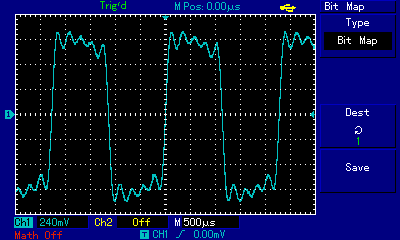
\includegraphics{content/MAP001.png}
\end{figure}
\begin{figure}[H]
    \centering
    \caption{Überlagerung der Oberwellen für die Dreiecksfunktion.}
    \label{fig:drei}
    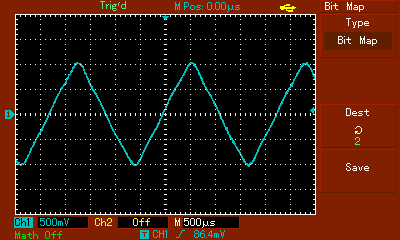
\includegraphics{content/MAP002.png}
\end{figure}
\begin{figure}[H]
    \centering
    \caption{Überlagerung der Oberwellen für die Sägezahnfunktion.}
    \label{fig:saeg}
    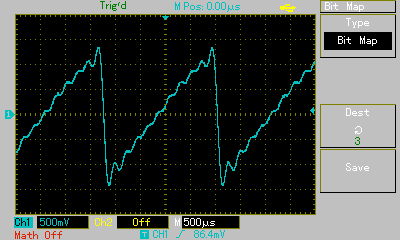
\includegraphics{content/MAP003.png}
\end{figure}
\noindent
Es wurden nur die ersten zehn Oberwellen verwendet um die hier aufgeführten Bilder zu erzeugen.
Die verwendeten Funktion werden durch die Überlagerung der Oberwellen annähernd approximiert.
